%%%%%%%%%%%%%%%%%%%%%%%%%%%%%%%%%%%%%%%%%%%%%%%%%%%%%%%%%%%%%%%%%%%%%%%%%%%%%%%%
%% Plantilla de memoria en LaTeX para la ETSIT - Universidad Rey Juan Carlos
%%
%% Por Gregorio Robles <grex arroba gsyc.urjc.es>
%%     Grupo de Sistemas y Comunicaciones
%%     Escuela Técnica Superior de Ingenieros de Telecomunicación
%%     Universidad Rey Juan Carlos
%% (muchas ideas tomadas de Internet, colegas del GSyC, antiguos alumnos...
%%  etc. Muchas gracias a todos)
%%
%% La última versión de esta plantilla está siempre disponible en:
%%     https://github.com/gregoriorobles/plantilla-memoria
%%
%% Para obtener PDF, ejecuta en la shell:
%%   make
%% (las imágenes deben ir en PNG o JPG)

%%%%%%%%%%%%%%%%%%%%%%%%%%%%%%%%%%%%%%%%%%%%%%%%%%%%%%%%%%%%%%%%%%%%%%%%%%%%%%%%

\documentclass[a4paper, 12pt]{book}
%\usepackage[T1]{fontenc}

\usepackage[a4paper, left=2.5cm, right=2.5cm, top=3cm, bottom=3cm]{geometry}
\usepackage{times}
\usepackage[utf8]{inputenc}
\usepackage[spanish]{babel} % Comenta esta línea si tu memoria es en inglés
\usepackage{url}
%\usepackage[dvipdfm]{graphicx}
\usepackage{graphicx}
\usepackage{float}  %% H para posicionar figuras
\usepackage[nottoc, notlot, notlof, notindex]{tocbibind} %% Opciones de índice
\usepackage{latexsym}  %% Logo LaTeX

\title{Memoria del Proyecto}
\author{Nombre del autor}

\renewcommand{\baselinestretch}{1.5}  %% Interlineado

\begin{document}

\renewcommand{\refname}{Bibliografía}  %% Renombrando
\renewcommand{\appendixname}{Apéndice}

%%%%%%%%%%%%%%%%%%%%%%%%%%%%%%%%%%%%%%%%%%%%%%%%%%%%%%%%%%%%%%%%%%%%%%%%%%%%%%%%
% PORTADA

\begin{titlepage}
\begin{center}
\includegraphics[scale=0.8]{img/URJ_logo_Color_POS.png}

\vspace{1.75cm}

\Large
GRADO EN INGENIERÍA EN SISTEMAS AUDIOVISUALES Y MULTIMEDIA

\vspace{0.4cm}

\large
Curso Académico 2021/2022

\vspace{0.8cm}

Trabajo Fin de Grado

\vspace{2.5cm}

\LARGE
IMPLEMENTACIÓN DE FUNCIONALIDADES EN LEARNINGML: RECONOCIMIENTO DE CONJUNTOS DE DATOS (DATASETS)

\vspace{3cm}

\large
Autor : Ignacio Rueda Rodríguez \\
Tutor : Dr. Gregorio Robles Martínez \\
Co-tutor : Juan David Rodríguez García
\end{center}
\end{titlepage}

\newpage
\mbox{}
\thispagestyle{empty} % para que no se numere esta pagina


%%%%%%%%%%%%%%%%%%%%%%%%%%%%%%%%%%%%%%%%%%%%%%%%%%%%%%%%%%%%%%%%%%%%%%%%%%%%%%%%
%%%% Para firmar
\clearpage
\pagenumbering{gobble}
\chapter*{}

\vspace{-4cm}
\begin{center}
\LARGE
\textbf{Trabajo Fin de Grado}

\vspace{1cm}
\large
Implementación de Funcionalidades en LearningML: Reconocimiento de Conjuntos de Datos (Datasets)

\vspace{1cm}
\large
\textbf{Autor :} Ignacio Rueda Rodríguez \\
\textbf{Tutor :} Dr. Gregorio Robles Martínez \\
\textbf{Co-tutor :} Juan David Rodríguez García

\end{center}

\vspace{1cm}
La defensa del presente Proyecto Fin de Carrera se realizó el día \qquad$\;\,$ de \qquad\qquad\qquad\qquad \newline de 2022, siendo calificada por el siguiente tribunal:


\vspace{0.5cm}
\textbf{Presidente:}

\vspace{1.2cm}
\textbf{Secretario:}

\vspace{1.2cm}
\textbf{Vocal:}


\vspace{1.2cm}
y habiendo obtenido la siguiente calificación:

\vspace{1cm}
\textbf{Calificación:}


\vspace{1cm}
\begin{flushright}
Fuenlabrada, a \qquad$\;\,$ de \qquad\qquad\qquad\qquad de 2022
\end{flushright}

%%%%%%%%%%%%%%%%%%%%%%%%%%%%%%%%%%%%%%%%%%%%%%%%%%%%%%%%%%%%%%%%%%%%%%%%%%%%%%%%
%%%% Dedicatoria

\chapter*{}
\pagenumbering{Roman} % para comenzar la numeracion de paginas en numeros romanos
\begin{flushright}
\textit{Dedicado a \\
mi familia, abuelos y amigos}
\end{flushright}

%%%%%%%%%%%%%%%%%%%%%%%%%%%%%%%%%%%%%%%%%%%%%%%%%%%%%%%%%%%%%%%%%%%%%%%%%%%%%%%%
%%%% Agradecimientos

\chapter*{Agradecimientos}
%\addcontentsline{toc}{chapter}{Agradecimientos} % si queremos que aparezca en el índice
\markboth{AGRADECIMIENTOS}{AGRADECIMIENTOS} % encabezado 

Aquí vienen los agradecimientos\ldots Aunque está bien acordarse de la pareja, no hay que olvidarse de dar las gracias a tu madre, que aunque a veces no lo parezca disfrutará tanto de tus logros como tú\ldots 
Además, la pareja quizás no sea para siempre, pero tu madre sí.

%%%%%%%%%%%%%%%%%%%%%%%%%%%%%%%%%%%%%%%%%%%%%%%%%%%%%%%%%%%%%%%%%%%%%%%%%%%%%%%%
%%%% Resumen

\chapter*{Resumen}
%\addcontentsline{toc}{chapter}{Resumen} % si queremos que aparezca en el índice
\markboth{RESUMEN}{RESUMEN} % encabezado

Aquí viene un resumen del proyecto.
Ha de constar de tres o cuatro párrafos, donde se presente de manera clara y concisa de qué va el proyecto. 
Han de quedar respondidas las siguientes preguntas:

\begin{itemize}
  \item ¿De qué va este proyecto? ¿Cuál es su objetivo principal?
  \item ¿Cómo se ha realizado? ¿Qué tecnologías están involucradas?
  \item ¿En qué contexto se ha realizado el proyecto? ¿Es un proyecto dentro de un marco general?
\end{itemize}

Lo mejor es escribir el resumen al final.

%%%%%%%%%%%%%%%%%%%%%%%%%%%%%%%%%%%%%%%%%%%%%%%%%%%%%%%%%%%%%%%%%%%%%%%%%%%%%%%%
%%%% Resumen en inglés

\chapter*{Summary}
%\addcontentsline{toc}{chapter}{Summary} % si queremos que aparezca en el índice
\markboth{SUMMARY}{SUMMARY} % encabezado

Here comes a translation of the ``Resumen'' into English. 
Please, double check it for correct grammar and spelling.
As it is the translation of the ``Resumen'', which is supposed to be written at the end, this as well should be filled out just before submitting.


%%%%%%%%%%%%%%%%%%%%%%%%%%%%%%%%%%%%%%%%%%%%%%%%%%%%%%%%%%%%%%%%%%%%%%%%%%%%%%%%
%%%%%%%%%%%%%%%%%%%%%%%%%%%%%%%%%%%%%%%%%%%%%%%%%%%%%%%%%%%%%%%%%%%%%%%%%%%%%%%%
% ÍNDICES %
%%%%%%%%%%%%%%%%%%%%%%%%%%%%%%%%%%%%%%%%%%%%%%%%%%%%%%%%%%%%%%%%%%%%%%%%%%%%%%%%

% Las buenas noticias es que los índices se generan automáticamente.
% Lo único que tienes que hacer es elegir cuáles quieren que se generen,
% y comentar/descomentar esa instrucción de LaTeX.

%%%% Índice de contenidos
\tableofcontents 
%%%% Índice de figuras
\cleardoublepage
%\addcontentsline{toc}{chapter}{Lista de figuras} % para que aparezca en el indice de contenidos
\listoffigures % indice de figuras
%%%% Índice de tablas
%\cleardoublepage
%\addcontentsline{toc}{chapter}{Lista de tablas} % para que aparezca en el indice de contenidos
%\listoftables % indice de tablas


%%%%%%%%%%%%%%%%%%%%%%%%%%%%%%%%%%%%%%%%%%%%%%%%%%%%%%%%%%%%%%%%%%%%%%%%%%%%%%%%
%%%%%%%%%%%%%%%%%%%%%%%%%%%%%%%%%%%%%%%%%%%%%%%%%%%%%%%%%%%%%%%%%%%%%%%%%%%%%%%%
% INTRODUCCIÓN %
%%%%%%%%%%%%%%%%%%%%%%%%%%%%%%%%%%%%%%%%%%%%%%%%%%%%%%%%%%%%%%%%%%%%%%%%%%%%%%%%

\cleardoublepage
\chapter{Introducción}
\label{sec:intro} % etiqueta para poder referenciar luego en el texto con ~\ref{sec:intro}
\pagenumbering{arabic} % para empezar la numeración de página con números

En este capítulo se introduce el proyecto.
Debería tener información general sobre el mismo, dando la información sobre el contexto en el que se ha desarrollado.

No te olvides de echarle un ojo a la página con los cinco errores de escritura más frecuentes\footnote{\url{http://www.tallerdeescritores.com/errores-de-escritura-frecuentes}}.

Aconsejo a todo el mundo que mire y se inspire en memorias pasadas.
Las memorias de los proyectos que he llevado yo están (casi) todas almacenadas en mi web del GSyC\footnote{\url{https://gsyc.urjc.es/~grex/pfcs/}}.

Dado que hoy 

\section{Sección}
\label{sec:seccion}

Esto es una sección, que es una estructura menor que un capítulo. 

Por cierto, a veces me comentáis que no os compila por las tildes.
Eso es un problema de codificación.
Al guardar el archivo, guardad la codificación de ``ISO-Latin-1'' a ``UTF-8'' (o viceversa) y funcionará.

\subsection{Estilo}
\label{subsec:estilo}

Recomiendo leer los consejos prácticos sobre escribir documentos científicos en \LaTeX \ de Diomidis Spinellis\footnote{\url{https://github.com/dspinellis/latex-advice}}.

Lee sobre el uso de las comas\footnote{\url{http://narrativabreve.com/2015/02/opiniones-de-un-corrector-de-estilo-11-recetas-para-escribir-correctamente-la-coma.html}}. 
Las comas en español no se ponen al tuntún.
Y nunca, nunca entre el sujeto y el predicado (p.ej. en ``Yo, hago el TFG'' sobre la coma).
La coma no debe separar el sujeto del predicado en una oración, pues se cortaría la secuencia natural del discurso.
No se considera apropiado el uso de la llamada coma respiratoria o \emph{coma criminal}.
Solamente se suele escribir una coma para marcar el lugar que queda cuando omitimos el verbo de una oración, pero es un caso que se da de manera muy infrecuente al escribir un texto científico (p.ej. ``El Real Madrid, campeón de Europa'').

A continuación, viene una figura, la Figura~\ref{figura:foro_hilos}. 
Observarás que el texto dentro de la referencia es el identificador de la figura (que se corresponden con el ``label'' dentro de la misma). 
También habrás tomado nota de cómo se ponen las ``comillas dobles'' para que se muestren correctamente. 
Nota que hay unas comillas de inicio (``) y otras de cierre (''), y que son diferentes.
Volviendo a las referencias, nota que al compilar, la primera vez se crea un diccionario con las referencias, y en la segunda compilación se ``rellenan'' estas referencias. 
Por eso hay que compilar dos veces tu memoria.
Si no, no se crearán las referencias.

 \begin{figure}
    \centering
    \includegraphics[bb=0 0 800 600, width=12cm, keepaspectratio]{img/foro1}
    \caption{Página con enlaces a hilos}
    \label{figura:foro_hilos}
 \end{figure}

A continuación un bloque ``verbatim'', que se utiliza para mostrar texto tal cual.
Se puede utilizar para ofrecer el contenido de correos electrónicos, código, entre otras cosas.

{\footnotesize
\begin{verbatim}
    From gaurav at gold-solutions.co.uk  Fri Jan 14 14:51:11 2005
    From: gaurav at gold-solutions.co.uk (gaurav_gold)
    Date: Fri Jan 14 19:25:51 2005
    Subject: [Mailman-Users] mailman issues
    Message-ID: <003c01c4fa40$1d99b4c0$94592252@gaurav7klgnyif>

    Dear Sir/Madam,
    How can people reply to the mailing list?  How do i turn off
    this feature? How can i also enable a feature where if someone
    replies the newsletter the email gets deleted?
    Thanks

    From msapiro at value.net  Fri Jan 14 19:48:51 2005
    From: msapiro at value.net (Mark Sapiro)
    Date: Fri Jan 14 19:49:04 2005
    Subject: [Mailman-Users] mailman issues
    In-Reply-To: <003c01c4fa40$1d99b4c0$94592252@gaurav7klgnyif>
    Message-ID: <PC173020050114104851057801b04d55@msapiro>

    gaurav_gold wrote:
    >How can people reply to the mailing list?  How do i turn off
    this feature? How can i also enable a feature where if someone
    replies the newsletter the email gets deleted?

    See the FAQ
    >Mailman FAQ: http://www.python.org/cgi-bin/faqw-mm.py
    article 3.11
\end{verbatim}
}

\section{Estructura de la memoria}
\label{sec:estructura}

En esta sección se debería introducir la esctura de la memoria. 

Así:

\begin{itemize}
  \item En el primer capítulo se hace una intro al proyecto.
  
  \item En el capítulo~\ref{chap:objetivos} (ojo, otra referencia automática) se muestran los objetivos del proyecto.
  
  \item A continuación se presenta el estado del arte en el capítulo~\ref{chap:estado}.
  
  \item \ldots
\end{itemize}



%%%%%%%%%%%%%%%%%%%%%%%%%%%%%%%%%%%%%%%%%%%%%%%%%%%%%%%%%%%%%%%%%%%%%%%%%%%%%%%%
%%%%%%%%%%%%%%%%%%%%%%%%%%%%%%%%%%%%%%%%%%%%%%%%%%%%%%%%%%%%%%%%%%%%%%%%%%%%%%%%
% OBJETIVOS %
%%%%%%%%%%%%%%%%%%%%%%%%%%%%%%%%%%%%%%%%%%%%%%%%%%%%%%%%%%%%%%%%%%%%%%%%%%%%%%%%

\cleardoublepage % empezamos en página impar
\chapter{Objetivos} % título del capítulo (se muestra)
\label{chap:objetivos} % identificador del capítulo (no se muestra, es para poder referenciarlo)

\section{Objetivo general} % título de sección (se muestra)
\label{sec:objetivo-general} % identificador de sección (no se muestra, es para poder referenciarla)

El trabajo fin de grado consiste en añadir a la aplicación web LearningML el reconocimiento de bases de datos.

Recuerda que los objetivos siempre vienen en infinitivo.


\section{Objetivos específicos}
\label{sec:objetivos-especificos}

Los objetivos específicos se pueden entender como las tareas en las que se ha desglosado el objetivo general.
Y, sí, también vienen en infinitivo.


\section{Planificación temporal}
\label{sec:planificacion-temporal}

A mí me gusta que aquí pongáis una descripción de lo que os ha llevado realizar el trabajo.
Hay gente que añade un diagrama de GANTT.
Lo importante es que quede claro cuánto tiempo llevas (tiempo natural, p.ej., 6 meses) y a qué nivel de esfuerzo (p.ej., principalmente los fines de semana).


%%%%%%%%%%%%%%%%%%%%%%%%%%%%%%%%%%%%%%%%%%%%%%%%%%%%%%%%%%%%%%%%%%%%%%%%%%%%%%%%
%%%%%%%%%%%%%%%%%%%%%%%%%%%%%%%%%%%%%%%%%%%%%%%%%%%%%%%%%%%%%%%%%%%%%%%%%%%%%%%%
% ESTADO DEL ARTE %
%%%%%%%%%%%%%%%%%%%%%%%%%%%%%%%%%%%%%%%%%%%%%%%%%%%%%%%%%%%%%%%%%%%%%%%%%%%%%%%%

\cleardoublepage
\chapter{Estado del arte}
\label{chap:estado}

\section{Inteligencia Artificial} 
\label{sec:InteligenciaArtificial}

La IA (\emph{Inteigencia Artificial})~\cite{rouhiainen2018inteligencia} se puede definir como la habilidad de los ordenadores para hacer actividades que normalmente requieren inteligencia humana. Aunque de forma más técnica se puede definir como la capacidad de las máquinas para usar algoritmos, aprender de los datos y utilizar lo aprendido en la toma de decisiones como si se tratase de un humano.

El uso de la IA cada vez es mayor, ya que nos ayuda a beneficiarnos de mejoras significativas y disfrutar de una mayor eficiencia en casi todos los ámbitos de la vida. Pero debemos estar atentos para prevenir y analizar las posibles desventajas directas o indirectas que pueda generar el crecimiento del uso de la IA. La IA se puede aplicar a una inmensidad de situaciones, algunas de ellas son las siguientes:

\begin{itemize}

    \item[•] Cambiará la forma de hacer negocios debido a que las empresas que busquen entender y aplicar estas herramientas de forma rápida y eficaz obtendrán ventajas competitivas. Por ejemplo, mejoras del desempeño de la estrategia algorítmica comercial o detección y clasificación de objetos.
    
	\item[•] La IA será capaz de ofrecernos sugerencias y predicciones relacionadas con temas importantes de nuestra vida, esto supondrá un impacto en áreas como la salud, el bienestar, la educación, el trabajo y las relaciones interpersonales. Por ejemplo, el procesamiento eficiente y escalable de datos de pacientes implicará que la atención médica sea
más efectiva y eficiente. 

	\item[•] Permitirá que las máquinas y los robots realicen tareas que los humanos consideran difíciles, aburridas o peligrosas. Además que las máquinas no necesitan descansar y pueden analizar grandes volúmenes de información a la vez y con un porcentaje de error menor que los humanos.
	
\end{itemize}

\section{Machine Learning} 
\label{sec:MachineLearning}
El machine learning o aprendizaje automático~\cite{rouhiainen2018inteligencia}  es uno de los enfoques fundamentales de la inteligencia artificial. Trata un elemento de la informática en el que los ordenadores o las máquinas tienen la capacidad de aprender sin estar programados para ello. El aprendizaje automático usa algoritmos para aprender de diferentes patrones de datos, es decir, es un conjunto de algoritmos con los que se construyen modelos de predicción y clasificación a partir de conjuntos de datos. Un ejemplo es la personalización de los sitios de medios sociales como Facebook o los resultados del motor de
búsqueda de Google. Otro ejemplo son  los filtros de Spam en el correo electronico. Aprenden en base a unos patrones que tipo de mensajes son correo basura y cuales no y toman la decision de clasificarlos como tal o no.

En el aprendizaje automático se diferencian tres tipos de aprendizaje:

\begin{itemize}

	\item[•] \textbf{Aprendizaje supervisado:} es el humano quien tiene que suministrar datos etiquetados y organizados para indicar cómo tendría que ser categorizada la nueva información o entrada. Por ejemplo, enseñar previamente al algoritmo fotos donde aparezca un perro para que luego pueda identificar imágenes similares. Es el tipo de aprendizaje utilizado en LearningML.
	
	\item[•] \textbf{Aprendizaje no supervisado:} es el algoritmo el que tiene que encontrar la forma de asignar a los datos una etiqueta sin información previa, de manera que no precisa de la intervención de un humano.
	
	\item[•] \textbf{Aprendizaje por refuerzo:} el algoritmo aprende de la experiencia. Cuando el algoritmo acierta al clasificar una entrada recibe un refuerzo positivo y de esta forma mejora con el uso.
	
\end{itemize}

\section{LearningML} 
\label{sec:LearningML}

LearningML~\cite{Pagina_de_LearningML} es una aplicación web creada por Juan David Rodríguez García en 2020, pero fué en 2019 cuando al autor decidió crear LearningML al participar en la confección de un recurso educativo\footnote{\url{https://code.intef.es/prop_didacticas/inteligencia-artificial-en-el-aula-con-scratch-3-0}}  sobre la enseñanza del aprendizaje automático en la escuela. La idea de crear LearningML surge porque la mayoría de las plataformas educativas de programación existentes carecen de algunas características necesarias para desarrollar proyectos completos de IA.

La aplicación web consiste en facilitar la enseñanza de contenidos sobre el aprendizaje automático y el fomento del pensamiento computacional a alumnos de edades comprendidas entre los 10 y los 16 años. Para comprobar si era una 
herramienta válida para enseñar, aprender machine learning y de uso sencillo se llevó a cabo una investigación\footnote{\url{https://web.learningml.org/investigacion-sobre-learningml/}} que resultó satisfactoria. En la actualidad, es una herramienta que está siendo utilizada en ambientes educativos reales.

Hoy en día LearningML dispone de dos funcionalidades básicas, reconocimiento de textos y reconocimiento de imágenes. Además cuenta con una amplia traducción a distintos idiomas.

\section{Angular} 
\label{sec:Angular}

Angular~\cite{Pagina_de_angular, Curso_de_angular} nació en 2010 con el nombre de AngularJS pero en el año 2016 pasó a llamarse Angular, en su versión 2.0 y ha ido evolucionando e implantando mejoras. La última versión es la 13 publicada en noviembre de 2021.

Angular es un \emph{framework} de código abierto desarrollado por Google que mediante el uso de TypeScript y HTML permite crear aplicaciones de una sola página, denominadas SPA (\emph{Single Page Application}).

Las ventajas que tiene Angular es que mantiene la aplicación más ordenada, simplifica el codigo y evita escribir código repetitivo gracias a que sigue un modelo MVC (\emph{Modelo-Vista-Controlador}), a la vez que posibilita que las modificaciones y las actualizaciones de las aplicaciones sean rápidas y sencillas. Además separa el \emph{frontend} y el \emph{backend} en la aplicación.

La principal ventaja que tienen las SPA es que tiene una alta velocidad de carga entre las vistas que tiene la aplicación web, ya que cuando hay un cambio de vista no se recarga la página si no que las vistas se cargan de forma rápida, dinámica y reactiva. Esto se debe a que solamente hay una petición inicial al servidor y una respuesta HTML del mismo, luego funciona mediante routing.

Como cualquier \emph{framework}, Angular tiene una serie de librerías que podemos
importar para facilitar el desarrollo del código, o para solucionar problemas
concretos. Las librerías amplían las funcionalidades.

La arquitectura de una aplicación Angular está basada en cuatro clases distintas, que se identifican a través de decoradores. Estos decoradores definen su tipo y proporcionan metadatos que le indican a Angular cómo usarlos.
Las cuatro clases que utiliza son:

\begin{itemize}

	\item[•] \textbf{Módulos:} declaran un contexto de compilación para un conjunto de componentes. Los módulos juegan un papel fundamental en la estructuración de las aplicaciones Angular. Es donde se definen o declaran los componentes, las directivas y los sevicios que conforman la aplicación. De manera que representa una agrupación lógica de lo que podríamos llamar áreas funcionales de una aplicación. También definen las rutas que establecen las vistas de la aplicación y las dependencias con otros módulos, es decir, que módulos necesita importar y que componentes o directivas exporta. 
	
	Cualquier aplicación de Angular tiene un módulo raiz, llamado \texttt{AppModule}, que proporciona el mecanismo de arranque que inicia la aplicación, pero no es el único, normalmente una aplicación contiene varios módulos funcionales, además de los propios del \emph{framework}. 
	
	Los módulos de Angular pueden importar o exportar funcionalidades de otros módulos, esto hace que cada módulo sea independiente. La organización en distintos módulos ayuda a gestionar el desarrollo de aplicaciones complejas y a la reutilización de código.
	
	Para definir una clase como módulo se utiliza el decorador \texttt{@NgModule}.
	
	\item[•] \textbf{Componentes:} son los bloques de construcción que componen una aplicación, contienen la lógica y los datos de la aplicación. Cada componente tiene asociada una plantilla HTML. Las plantillas son las vistas que conforman la interfaz de usuario y se cargan cuando se cambia o modifica la URL.
	
	Una aplicación de Angular tiene al menos el componente raiz, llamado \texttt{AppComponent}, que conecta una jerarquía de componentes con el modelo de objeto del documento (DOM) de la página.
	
	Los componentes pueden tener uno o varios subcomponentes, estos pueden relacionarse entre sí de dos formas. Mediante eventos para actualizar datos cuando el usuario interacciona con la interfaz grafica y mediante las propiedades o interpolación para enviar datos a las plantillas que conforman las vistas. Esto hace que los cambios en el DOM pueden modificar los datos de la aplicación y los datos de la aplicación pueden modificar las plantillas.
	
	Para definir una clase como componente se utiliza el decorador \texttt{@NgComponent}.
	
	\item[•] \textbf{Directivas:} son clases que agregan comportamiento adicional a los elementos en sus aplicaciones Angular para modificar de alguna manera el HTML. Antes de que se muestre una vista, Angular evalúa las directivas y resuelve la sintaxis vinculante en la plantilla para modificar los elementos HTML y el DOM.
	
	Hay tres tipos de directivas:
	
	\begin{itemize}
	\item[*] Directivas de componente: los componentes son un tipo de directiva.
	\item[*] Directivas de atributos: modifican el comportamiento o la apariencia de un elemento, componente o directiva.
	\item[*] Directivas estructuales: modifican la apariencia agregando y eliminando elementos del DOM.
	\end{itemize}
	
	Se pueden crear directivas o Angular dispone de directivas integradas que se pueden usar para administrar formularios, listas, estilos y lo que ven los usuarios. Algunos ejemplos de directivas de atributos integradas son \texttt{NgClass}, \texttt{NgStyle} y \texttt{NgModel}, y de directivas estructurales \texttt{NgIf}, \texttt{NgFor} y \texttt{NgSwitch}.
	
	\item[•] \textbf{Servicios:} proporcionan una funcionalidad específica que no está directamente relacionada con las vistas. Son clases con un propósito limitado y bien definido, deben hacer algo específico y de uso general. Se usan para cambiar datos entre componentes, obtener datos del servidor, validar la entrada del usuario o cualquier servicio que se repita en distintas componentes.
	
	Angular distingue los componentes de los servicios para aumentar la modularidad y la reutilización. Al separar la funcionalidad relacionada con la vista de un componente de otros tipos de procesamiento, puede hacer que sus clases de componentes sean sencillas y eficientes.
	
	Para definir una clase como servicio se utiliza el decorador \texttt{@Injectable},ya que proporciona los metadatos que permiten inyectar otros proveedores como dependencias en su clase.
	
\end{itemize}


\subsection{Angular CLI}
\label{subsec:Angular CLI}

Angular CLI (\emph{Command Line Interface})~\cite{Pagina_de_angular_CLI} es una herramienta de interfaz de línea de comandos desarrollada por Angular que se utiliza para inicializar, desarrollar, montar y mantener aplicaciones de Angular directamente desde un shell de comandos. 

Es una herramienta que facilita el inicio de una aplicación de Angular, porque con una instrucción \texttt{ngnew}, crea una carpeta de trabajo y genera el esqueleto de aplicación. También tiene instrucciones que permiten crear nuevas clases de forma sencilla, creando los distintos archivos que forman un módulo, componente, servicio o una directiva, además de incluirlos en los archivos necesrios y crear las dependencias. Las herramientas predefinidas más destacadas son el servidor web, el compilador y el sistema de testing.


\subsection{MVC}
\label{subsec:MVC}

Para el desarrollo de una aplicación web Angular utiliza el patrón MVC (\emph{Modelo-Vista-Controlador})~\cite{Pagina_MVC} que se utiliza para separar en tres componentes los datos, la metodología y la interfaz gráfica de una aplicación, lo que permite modificar cada uno de ellos sin tener que modificar los demas. La arquitectura MVC está formada por tres componentes, que son:
	\begin{itemize}
	\item[•] \textbf{Modelo:} es el encargado de la manipulación, gestión y actualización de los datos. En el caso de que haya una base de datos es donde se realizan las consultas, busquedas o actualizaciones.  
	
	\item[•] \textbf{Vista:} es la representación gráfica de los datos proporcionados por el controlador. Ni el controlador ni el modelo se preocupan de cómo se verán los datos, toda la parte del diseño de la interfaz es responsabilidad de la vista.
	
	\item[•] \textbf{Controlador:} es el componente principal, se encarga de gestionar las instrucciones que se reciben del usuario, atenderlas y procesarlas. Después realiza las consultas al modelo y una vez se hayan obtenido dichos datos, se envía a la vista para producir una salida como respuesta a el evento.
	\end{itemize}
	
Las ventajas que aporta esta arquitectura son:facilita el mantenimiento, permite la reutilización de componentes y mejora la escalabilidad, ya que separa cada tipo de lógica.


\section{HTML5} 
\label{sec:HTML5}

HTML (\emph{HyperText Markup Language})~\cite{Pagina_HTML, Historia_HTML5, gauchat2012gran} es un lenguaje de marcado que se utiliza para definir la estructura y el contenido de una página Web, y es el componente más básico de una web. Se escribe en texto plano y tiene una estructura de árbol de elementos y textos. La estructura básica de un documento HTML se compone de los siguientes elementos: \texttt{<!DOCTYPE>}, \texttt{<html>}, \texttt{<head>} y \texttt{<body>}. HTML provee los elementos estructurales y se complemeta con CSS para modificar la apariencia de la pagina y con JavaScript para proveer dinamismo y construir aplicaciones web completamente funcionales. 

La idea de desarrollar HTML5 nació en 2004, cuando el consorcio W3C (\emph{World Wide Web Consortium})  que está a cargo del estandar deció dejar de evolucionar HTML, por lo que la asociación WHATWG (\emph{Web HyperText Application Technology Working Group}), formada por Apple, Opera y Mozilla, decidió crear HTML5 y publicó el primer borrador de HTML5. En el año 2007 W3C formó un grupo de trabajo autorizado para trabajar con WHATWG en el desarrollo de HTML5, pero en 2011 se separaron debido a que tenían distintos objetivos, W3C quería publicar una version terminada, mientras que WHATWG quería seguir trabajando en una constante evolución de HTML5. En 2019, WHATWG y W3C firmaron un acuerdo para colaborar en una única versión de HTML en el futuro.

Fue creado con la intención de hacerlo más eficiente que las versiones anteriores, mantener la compatibilidad con versiones anteriores y facilitar el desarrollo web compatible con distintos navegadores. Las principales novedades de HTML5 son:

	\begin{itemize}
	\item[•] Incorpora nuevas etiquetas que permiten una mejor estructuración de los documentos HTML, ya que antes solo estaba el \texttt{<div>} para definir secciones. Ahora se pueden utilizar también \texttt{<header>} para la cabecera, \texttt{<section>} para la información principal, \texttt{<nav>} para la barra de navegación y \texttt{<footer>} para el pie, entre otros.
	\item[•] Permite incorporar elementos multimedia para reproducir audios y videos desde el propio navegador, con las etiquetas \texttt{<audio>} y \texttt{<video>}.
	\item[•] Incluye numerosas APIs, algunas de ellas son:
		\begin{itemize}
		\item[*] Forms: incluye mejoras en los formularios para personalizar todos los aspectos de procesamiento y validación.
		\item[*] Canvas: permite dibujar, presentar gráficos en pantalla, animar y procesar imágenes y texto.
		\item[*] Geolocation: permite a los desarrolladores determinar la ubicación física real del usuario y e mostrar e interactuar con un mapa de Google Maps.
		\item[*] Drag and drop: permite arrastrar un elemento desde un lugar y luego soltarlo en otro.
		\item[*] Web Storage: es una mejora de las cookies y permite el almacenamiento local en el lado del cliente, con \texttt{localStorage} cuando la información tiene que estar disponible solo durante la sesión y \texttt{sessionStorage} cuando tiene que ser preservada todo el tiempo que el usuario desee
		\end{itemize}
	\end{itemize}


\section{CSS3} 
\label{sec:CSS3}

CSS3 (\emph{Cascading Style Sheets})~\cite{gauchat2012gran} es la última versión de CSS. Es un lenguaje de diseño gráfico que permite definir y crear el aspecto visual de los documentos HTML. Es un complemento desarrollado para superar las limitaciones y reducir la complejidad de HTML, por lo que se separa el estilo del documento de la estructura y el contenido de este. Esta separación permite que varios documentos HTML tengan la misma hoja de estilo, simplificando el trabajo de los desarrolladores, o que un mismo documento HTML pueda tener distintos estilos, permitiendo variaciones en la visualización para diferentes dispositivos y tamaños de pantalla.

El consorcio W3C es el encargado de definir y mantener las especificaciones de este lenguaje. Las principales novedades de CSS3 son: esquinas redondeadas, sombras en cajas y textos, elegir la fuente del texto, gradientes, opacidad y transparencia de los colores, incluir transiciones, entre otras.

\section{TypeScript} 
\label{sec:TypeScript}

TypeScript~\cite{Pagina_de_typescript} es un lenguaje de programación de código abierto desarrollado y mantenido por Microsoft. Es un superconjunto de JavaScript, es decir, amplía JavaScript con una nueva sintaxis que añade tipos estáticos y objetos basados en clases. Nació en 2012 como solución para el desarrollo de aplicaciones  robustas y de gran tamano, ya que con JavaScript era muy complicado debido a su escasa escalabilidad. Su uso está permitido tanto en el lado del cliente como en el lado del servidor con Node.js

 Los programas de JavaScript son compatibles en TypeScript, por lo que se puede integrar en proyectos ya existentes porque a través de un compilador de TypeScript se traducen a código JavaScript original. Además tiene las herramientas de JavaScript ES6 y JavaScript ES7, de esta manera se mantiene actualizado con las últimas mejoras de JavaScript. Los cambios más importantes respecto a JavaScript son:

\begin{itemize}
	\item[•] Evita errores en tiempo de ejecución, ya que incorpora el tipado estático, es decir, al crear variables se puede añadir el tipo de dato.
	
	\item[•] Es más funcional, ya que al añadir objetos basados en clases hace que la programación orientada a objetos sea más sencilla
\end{itemize}

En la actualidad se encuentra en la versión 2.0 que introduce varias características, entre ellas la capacidad de evitar la asignación de variables con un valor nulo. 

\section{Node.js} 
\label{sec:Node}

Node.js~\cite{Pagina_de_Node} fue creado por Ryan Dahl en 2009. Es un entorno en tiempo de ejecución de JavaScript orientado a eventos asíncronos, diseñado para construir aplicaciones de red escalables, como por ejemplo, servidores web. Está influenciado por sistemas como Event Machine de Ruby y Twisted de Python.

Con Node.js el código JavaScript, no se ejecuta en un navegador, sino en el servidor. Utiliza el motor V8 de Google para interpretar y ejecutar el código JavaScript, suministrando un entorno de ejecución en el lado del servidor. Del mismo modo que hace el navegador cuando se utiliza JavaScript en el lado del cliente.

Al estar orientado a eventos asíncronos puede soportar una gran cantidad de conexiones. Esto lo diferencia del modelo de concurrencia más común, en el que se emplean hilos del Sistema Operativo que usan un hilo por cada conexión, lo que provoca que si se tienen muchas conexiones son necesarios muchos servidores. Node.js utiliza un único hilo de ejecución y un bucle de eventos asíncrono, tratando las nuevas conexiones como un nuevo evento dentro del bucle y cada conexión recibe una pequeña asignación de espacio de memoria dinámico, sin tener que crear un hilo de ejecución, evitando que se produzcan bloqueos en el flujo de trabajo. 

Node.js utiliza un único hilo de ejecución y un bucle de eventos asíncrono, tratando las nuevas conexiones como un nuevo evento dentro del bucle y cada conexión recibe una pequeña asignación de espacio de memoria dinámico, sin tener que crear un hilo de ejecución, de esta manera evita que se produzcan bloqueos en el flujo de trabajo y permite soportar una gran cantidad de conexiones. Esto lo diferencia del modelo de concurrencia más común, en el que se emplean hilos del Sistema Operativo que usan un hilo por cada conexión, lo que provoca que si se tienen muchas conexiones son necesarios muchos servidores.

\section{TensorFlow} 
\label{sec:TensorFlow}

TensorFlow~\cite{Pagina_de_TensorFlow} es el sistema de aprendizaje automático de segunda generación de Google Brain, liberado como software de código abierto en 2015, por lo que el acceso a esta herramienta es libre y es posible editarla en función de las necesidades. 

Es una plataforma para construir y entrenar redes neuronales para detectar y descifrar patrones y correlaciones, parecidos al aprendizaje y razonamiento usados por los humanos. Tiene un ecosistema integral y flexible de herramientas , bibliotecas y recursos de la comunidad que permite a los desarrolladores crear e implementar fácilmente aplicaciones basadas en ML.


\section{JSON} 
\label{sec:JSON}

JSON (\emph{JavaScript Object Notation})~\cite{Pagina_de_JSON} es un formato ligero de intercambio de datos. Es fácil de leer y escribir para los humanos, mientras que para las máquinas es sencillo de interpretar y generar. A pesar de que está basado en un subconjunto del lenguaje de programación JavaScript, es un formato de texto completamente independiente del lenguaje. JSON está construído por dos estructuras:

\begin{itemize}
	\item[•] Objeto: colección de pares de nombre/valor. Comienza con una llave de apertura y termina con una llave de cierre, cada nombre es seguido de dos puntos y los pares nombre/valor están separados por una coma.
	\item[•] Array: lista ordenada de valores. Comienza con un corchete izquierdo y termina con un corchete derecho, los valores se separan por comas.
\end{itemize}

Estas estructuras pueden anidarse y los valores pueden ser:
	\begin{itemize}
		\item[•] Cadena de caracteres. Se ponen entre comillas dobles.
		\item[•] Números. Pueden contener parte fraccional separada por un punto y se permiten números negativos.
		\item[•] Booleanos. True y false.
		\item[•] Null. Representa el valor nulo.
	\end{itemize}



%%%%%%%%%%%%%%%%%%%%%%%%%%%%%%%%%%%%%%%%%%%%%%%%%%%%%%%%%%%%%%%%%%%%%%%%%%%%%%%%
%%%%%%%%%%%%%%%%%%%%%%%%%%%%%%%%%%%%%%%%%%%%%%%%%%%%%%%%%%%%%%%%%%%%%%%%%%%%%%%%
% DISEÑO E IMPLEMENTACIÓN %
%%%%%%%%%%%%%%%%%%%%%%%%%%%%%%%%%%%%%%%%%%%%%%%%%%%%%%%%%%%%%%%%%%%%%%%%%%%%%%%%

\cleardoublepage
\chapter{Diseño e implementación} 

\section{Arquitectura de LearningML} 
\label{sec:arquitectura}

La arquitectura de LearningML está construida con Angular, por lo que está compuesta por módulos, componentes y servicios, de manera que es sencillo realizar cambios o añadir funcionalidades. 

En la figura~\ref{fig:arquitectura} se puede ver la arquitectura general de LearningML, primero está el servicio \texttt{labeled-data-manager}, es de uso general y lo importan la mayoría de componentes y algunos sevicios, ya que se encarga de guardar  algunos datos que necesitan los servicios y componentes. Luego está el componente \texttt{ml-home} que se corresponde con la página inicial y es donde se selecciona que tipo de reconocimiento se desea realizar, reconocimiento de textos o de imagenes. Una vez se ha seleccionado se pasa al componente \texttt{ml-model} mediante routing con el modelo \texttt{app-routing} que funciona mediante rutas, por lo que además de cambiar de componente también se cambia de página. En función del reconocimiento escogido se mostrarán unos elementos u otros del HTML de \texttt{ml-model}.

En el componente \texttt{ml-model} se importan los servicios \texttt{feature-extraction} y \texttt{ml-algorithm}, que a su vez el primero importa dos servicios: \texttt{feature-extractor-text} y \texttt{feature-extractor-
image} y el segundo importa otros dos servicios: \texttt{ml-algorithm-knn} y \texttt{ml-algorithm-
neural-networks}.

El componente \texttt{ml-model} es el contructor del modelo y está dividido en tres secciones, la primera es donde se introducen los datos de entrenamiento, primero se introducen las distintas clases a las que puede pertenecer una entrada y una vez se ha introducido al menos una clase, entra en funcionamiento el componente \texttt{ml-label-container} que es donde se recogen las entradas de cada clase con los datos que se utilizan en la segunda sección, la parte de aprendizaje. \\
En la parte de aprendizaje es donde se utiliza la función \texttt{train} que es donde realmente se realiza la construcción del modelo y se entrena, primero se realiza la extracción de características mediante el servicio \texttt{feature-extraction} y este es el que elige dependiendo del tipo de dato cual de los dos servicios usar para la extracción de características. Después llama a \texttt{ml-algorithm} y este servicio decide que algoritmo utilizar para construir y entrenar el modelo para el reconocimiento. Por defecto utiliza el algoritmo \texttt{ml-algorithm-neural-networks}, pero se puede seleccionar el modo avanzado en el cual se puede elegir entre los dos y modificar los parámetros del algoritmo.\\
Cuando el modelo ya está entrenado se pasa a la tercera sección, la parte de testeo, que es donde se realizan las pruebas de reconocimiento. En función del reconocimiento escogido se hace uso del componente \texttt{ml-test-text-model} o del componente \texttt{ml-test-image-model}. Primero llaman a \texttt{feature-extraction} y después a \texttt{ml-algorithm}, igual que \texttt{ml-model}.

\begin{figure}
	\centering
	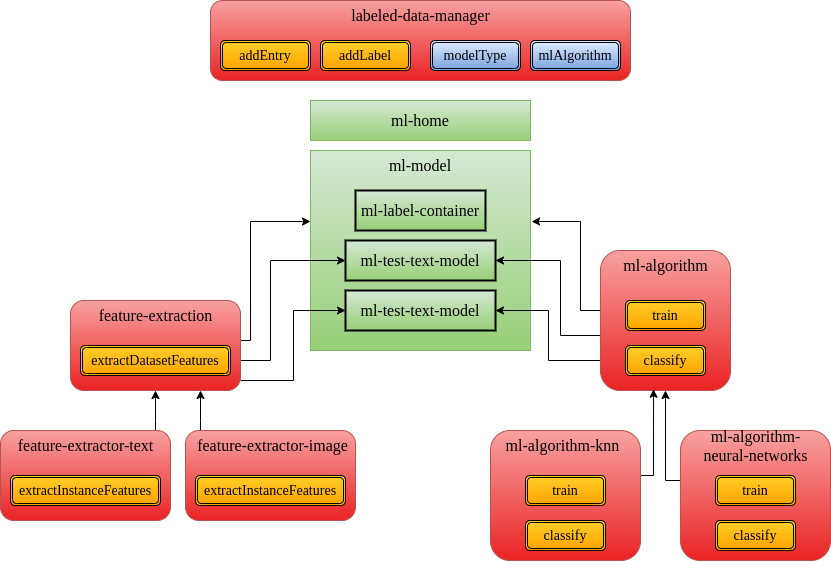
\includegraphics[width=12cm, keepaspectratio]{img/arquitectura.png}
	\caption{Arquitectura general de \texttt{LearningML}. En rojo los servicios, en verde los componentes, en amarillo las funciones y en azul las variables.} \label{fig:arquitectura}
\end{figure}

En la figura~\ref{fig:arquitectura} también se puede observar que contiene principalmente cada servicio nombrado anteriormente. Estos servicios tienen un desempeño específico:

\begin{itemize}
	\item[•] labeled-data-manager: es el encargado de guardar datos, estos datos son características que definen el modelo. Guarda las etiquetas, es decir, las clases a las que puede pertenecer una entrada, esto se hace con la función \texttt{addLabel} que guarda las etiquetas en un array llamado  \texttt{labels} y en un objeto Map llamado \texttt{labelsWithData}. Guarda los datos de entrada, ya sean textos o imágenes, con la función \texttt{addEntry} que los guarda en el objeto \texttt{labelsWithData} junto con la etiqueta de la clase en la que ha sido añadida la entrada para así tener cada etiqueta con sus datos. Guarda el tipo de modelo que se va a construir, es decir, el tipo de reconocimiento selecionado, en la variable \texttt{modelType}. También guarda el tipo de algoritmo en la variable \texttt{mlAlgorithm}. Además de guardar estos datos también borra etiquetas o entradas y se encarga de guardar o cargar los datos de un JSON tanto del ordenador como de la nube si el usuario está registrado.
	
	\item[•] feature-extraction: es el encargado de llamar a los otros dos servicios en función de si se quieren extraer características de un texto o de una imagen mediante la función \texttt{extractDatasetFeatures}.
	
	\begin{itemize}
		\item[*] feature-extractor-text: es el encargado de extraer las características de los textos, es decir, convertir un texto en un tensor. La función que lo convierte en un tensor es \texttt{extractInstanceFeatures}
		
		\item[*] feature-extractor-image: es el encargado de extraer las características de las imágenes, es decir, convertir una imagen en un tensor. La función que lo convierte en un tensor es \texttt{extractInstanceFeatures} al igual que en el caso de los textos.
	\end{itemize}
	
	\item[•] ml-algorithm: es el encargado de llamar a los otros dos servicios en función del algoritmo que se utilice. Tiene dos funciones principales, \texttt{train} y \texttt{classify} con las que llama a los otros servicios para entrenar o clasificar.
	
	\begin{itemize}
		\item[*] ml-algoithm-knn: se usa en caso de que el algoritmo elegido sea K-NN. Tiene dos funciones que son las que llama el servicio \texttt{ml-algorithm}, \texttt{train} para entrenar o \texttt{classify} para clasificar.
		\item[*] ml-algorithm-neural-networks: tiene las mismas funciones que K-NN pero en este caso entrena o evalúa utilizando el algoritmo de redes neuronales.
	\end{itemize}
\end{itemize}

\section{Cambios en la arquitectura de LearningML} 
\label{sec:arquitectura nueva}

Realizar cambios en la arquitectura no fue complicado, ya que la aplicación está hecha para poder realizar cambios e implementar nuevas funcionalidades. Solo hay que entender como esta estructurada y que es lo que hace cada parte.

Para añadir la nueva funcionalidad tenía dos opciones en cuanto a la construcción del modelo: crear un nuevo componente o añadir la funcionalidad en el componente \texttt{ml-model}, me decidí por la segunda para seguir con la misma estructura, ya que no había un componente diferente para construir el modelo de textos y otro para imágenes, por lo que me parecía más lógico seguir con la misma dinámica.




Aquí viene todo lo que has hecho tú (tecnológicamente). 
Puedes entrar hasta el detalle. 
Es la parte más importante de la memoria, porque describe lo que has hecho tú.
Eso sí, normalmente aconsejo no poner código, sino diagramas.

Si tu proyecto es un software, siempre es bueno poner la arquitectura (que es cómo se estructura tu programa a ``vista de pájaro'').

Por ejemplo, puedes verlo en la figura~\ref{fig:arquitectura}.
\LaTeX \ pone las figuras donde mejor cuadran. 
Y eso quiere decir que quizás no lo haga donde lo hemos puesto\ldots
Eso no es malo.
A veces queda un poco raro, pero es la filosofía de \LaTeX: tú al contenido, que yo me encargo de la maquetación.


\begin{figure}[b!]
    \centering 
    \includegraphics[bb=0 0 800 600, width=12cm, keepaspectratio]{img/foro1}
    \caption{Página con enlaces a hilos}\label{fig:_arquitectura}
\end{figure}

 
Recuerda que toda figura que añadas a tu memoria debe ser explicada.
Sí, aunque te parezca evidente lo que se ve en la figura~\ref{fig:arquitectura}, la figura en sí solamente es un apoyo a tu texto.
Así que explica lo que se ve en la figura, haciendo referencia a la misma tal y como ves aquí.
Por ejemplo: En la figura~\ref{fig:arquitectura} se puede ver que la estructura del \emph{parser} básico, que consta de seis componentes diferentes: los datos se obtienen de la red, y según el tipo de dato, se pasará a un \emph{parser} específico y bla, bla, bla\ldots

Si utilizas una base de datos, no te olvides de incluir también un diagrama de entidad-relación.


%%%%%%%%%%%%%%%%%%%%%%%%%%%%%%%%%%%%%%%%%%%%%%%%%%%%%%%%%%%%%%%%%%%%%%%%%%%%%%%%
%%%%%%%%%%%%%%%%%%%%%%%%%%%%%%%%%%%%%%%%%%%%%%%%%%%%%%%%%%%%%%%%%%%%%%%%%%%%%%%%
% EXPERIMENTOS Y VALIDACIÓN %
%%%%%%%%%%%%%%%%%%%%%%%%%%%%%%%%%%%%%%%%%%%%%%%%%%%%%%%%%%%%%%%%%%%%%%%%%%%%%%%%

\cleardoublepage
\chapter{Experimentos y validación}

Este capítulo se introdujo como requisito en 2019. 
Describe los experimentos y casos de test que tuviste que implementar para validar tus resultados. 
Incluye también los resultados de validación que permiten afirmar que tus resultados son correctos. 


%%%%%%%%%%%%%%%%%%%%%%%%%%%%%%%%%%%%%%%%%%%%%%%%%%%%%%%%%%%%%%%%%%%%%%%%%%%%%%%%
%%%%%%%%%%%%%%%%%%%%%%%%%%%%%%%%%%%%%%%%%%%%%%%%%%%%%%%%%%%%%%%%%%%%%%%%%%%%%%%%
% RESULTADOS %
%%%%%%%%%%%%%%%%%%%%%%%%%%%%%%%%%%%%%%%%%%%%%%%%%%%%%%%%%%%%%%%%%%%%%%%%%%%%%%%%

\cleardoublepage
\chapter{Resultados}

En este capítulo se incluyen los resultados de tu trabajo fin de grado.

Si es una herramienta de análisis lo que has realizado, aquí puedes poner ejemplos de haberla utilizado para que se vea su utilidad.


%%%%%%%%%%%%%%%%%%%%%%%%%%%%%%%%%%%%%%%%%%%%%%%%%%%%%%%%%%%%%%%%%%%%%%%%%%%%%%%%
%%%%%%%%%%%%%%%%%%%%%%%%%%%%%%%%%%%%%%%%%%%%%%%%%%%%%%%%%%%%%%%%%%%%%%%%%%%%%%%%
% CONCLUSIONES %
%%%%%%%%%%%%%%%%%%%%%%%%%%%%%%%%%%%%%%%%%%%%%%%%%%%%%%%%%%%%%%%%%%%%%%%%%%%%%%%%

\cleardoublepage
\chapter{Conclusiones}
\label{chap:conclusiones}


\section{Consecución de objetivos}
\label{sec:consecucion-objetivos}

Esta sección es la sección espejo de las dos primeras del capítulo de objetivos, donde se planteaba el objetivo general y se elaboraban los específicos.

Es aquí donde hay que debatir qué se ha conseguido y qué no. 
Cuando algo no se ha conseguido, se ha de justificar, en términos de qué problemas se han encontrado y qué medidas se han tomado para mitigar esos problemas.

Y si has llegado hasta aquí, siempre es bueno pasarle el corrector ortográfico, que las erratas quedan fatal en la memoria final.
Para eso, en Linux tenemos aspell, que se ejecuta de la siguiente manera desde la línea de \emph{shell}:

\begin{verbatim}
  aspell --lang=es_ES -c memoria.tex
\end{verbatim}

\section{Aplicación de lo aprendido}
\label{sec:aplicacion}

Aquí viene lo que has aprendido durante el Grado/Máster y que has aplicado en el TFG/TFM. Una buena idea es poner las asignaturas más relacionadas y comentar en un párrafo los conocimientos y habilidades puestos en práctica.

\begin{enumerate}
  \item a
  \item b
\end{enumerate}


\section{Lecciones aprendidas}
\label{sec:lecciones_aprendidas}

Aquí viene lo que has aprendido en el Trabajo Fin de Grado/Máster.

\begin{enumerate}
  \item Aquí viene uno.
  \item Aquí viene otro.
\end{enumerate}


\section{Trabajos futuros}
\label{sec:trabajos_futuros}

Ningún proyecto ni software se termina, así que aquí vienen ideas y funcionalidades que estaría bien tener implementadas en el futuro.

Es un apartado que sirve para dar ideas de cara a futuros TFGs/TFMs.


%%%%%%%%%%%%%%%%%%%%%%%%%%%%%%%%%%%%%%%%%%%%%%%%%%%%%%%%%%%%%%%%%%%%%%%%%%%%%%%%
%%%%%%%%%%%%%%%%%%%%%%%%%%%%%%%%%%%%%%%%%%%%%%%%%%%%%%%%%%%%%%%%%%%%%%%%%%%%%%%%
% APÉNDICE(S) %
%%%%%%%%%%%%%%%%%%%%%%%%%%%%%%%%%%%%%%%%%%%%%%%%%%%%%%%%%%%%%%%%%%%%%%%%%%%%%%%%

\cleardoublepage
\appendix
\chapter{Manual de usuario}
\label{app:manual}

Esto es un apéndice.
Si has creado una aplicación, siempre viene bien tener un manual de usuario.
Pues ponlo aquí.

%%%%%%%%%%%%%%%%%%%%%%%%%%%%%%%%%%%%%%%%%%%%%%%%%%%%%%%%%%%%%%%%%%%%%%%%%%%%%%%%
%%%%%%%%%%%%%%%%%%%%%%%%%%%%%%%%%%%%%%%%%%%%%%%%%%%%%%%%%%%%%%%%%%%%%%%%%%%%%%%%
% BIBLIOGRAFIA %
%%%%%%%%%%%%%%%%%%%%%%%%%%%%%%%%%%%%%%%%%%%%%%%%%%%%%%%%%%%%%%%%%%%%%%%%%%%%%%%%

\cleardoublepage

% Las siguientes dos instrucciones es todo lo que necesitas
% para incluir las citas en la memoria
\bibliographystyle{abbrv}
\bibliography{memoria}  % memoria.bib es el nombre del fichero que contiene
% las referencias bibliográficas. Abre ese fichero y mira el formato que tiene,
% que se conoce como BibTeX. Hay muchos sitios que exportan referencias en
% formato BibTeX. Prueba a buscar en http://scholar.google.com por referencias
% y verás que lo puedes hacer de manera sencilla.
% Más información: 
% http://texblog.org/2014/04/22/using-google-scholar-to-download-bibtex-citations/

\end{document}
